\section{Recommendations}
\label{sec:recommendations}

On analysing the root causes of each of the challenges, we assert that to realize the benefits of using formal methods to verify requirements we need adapt both the requirements engineering activities to support formal methods as well as the formal techniques to recognize common requirement verification concerns. In this section, we elaborate on how we addressed the first two challenges by changing requirements engineering process and the other two challenges by changing and enhancing the formal tools.

\subsection {Solution To Challenge 1: Structuring Requirements}

To systematically identify the context of each requirement and its dependencies with other requirements, we hierarchically restructured the GPCA requirement document as shown in Figure~\ref{fig:gpca-requirements}, that not only simplified the formalization process also helped understand the system in a conceptually clear way. The system behaviors of most control systems are typically captured by grouping them in terms of \emph{modes} - a logical way to describe a set of system behaviours. In a complex system, there could be many modes that could either be mutually exclusive (only one mode can be active at a time) or orthogonal (multiple modes can be active at a time). By grouping the modes based on their common and exclusive behaviours as well as their interactions, we hierarchically organized them that helped systematically documenting, formalizing and verifying the requirements.

 \begin{figure}[h!]
    \centering
    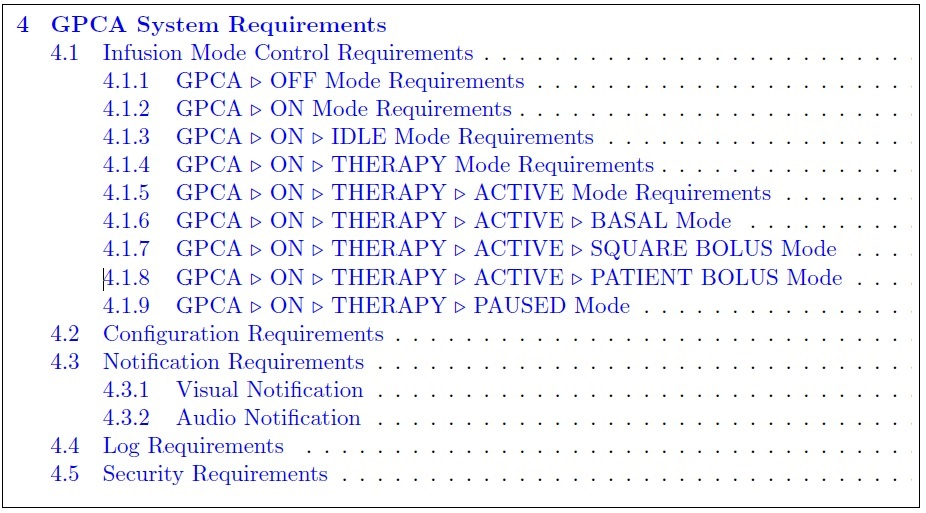
\includegraphics[width=\columnwidth]{images/structuring.jpg}
    \caption{GPCA System Requirements Structuring}
    \label{fig:gpca-requirements}
 \end{figure}

In the GPCA, there were three main orthogonal groups of modes - infusion, configuration and notification modes. Within each orthogonal group, there were a set of modes that were mutually exclusive to each other such as basal, intermittent and patient bolus modes within infusion mode group. Similarly, the notification group had 18 requirements that we further categorized based on its severity level (Levels 4 to 1). When we analysed the requirements, we understood that there were many requirements that were common to the exclusive modes among an orthogonal group, as well as requirements that were common to all the three orthogonal mode groups. We leveraged this pattern of modal requirements to organize requirement statements within the document in an hierarchial fashion. In this structuring, at the top most level we placed requirements that were common to the entire system. At the next level, we placed the mode groups that were orthogonal to each other. Within each orthogonal mode group, we again followed the hierarchical structure to organize their requirements. For clarity purposes, within a mode group we grouped requirements hierarchically based on their behaviours and named it as a new mode (although it was not explicitly mentioned by the stakeholders). For example, we placed all the requirements that were common among the basal and boluses infusions in a parent mode called \emph{Therapy} mode and made the basal and bolus its child modes with its own set of special requirements. For additional clarity on understanding the mutual exclusivity among modal behaviours, we documented requirements using a tabular notation. An example of the tabular format we used for the notification requirements is shown in Figure~\ref{fig:gpca-alarm}. Although we came across a couple of requirements that had minor variations to be grouped, this structuring helped identify those differences and we were able to clearly negotiate with our domain experts on appropriately categorizing them. 

 \begin{figure}[h!]
    \centering
    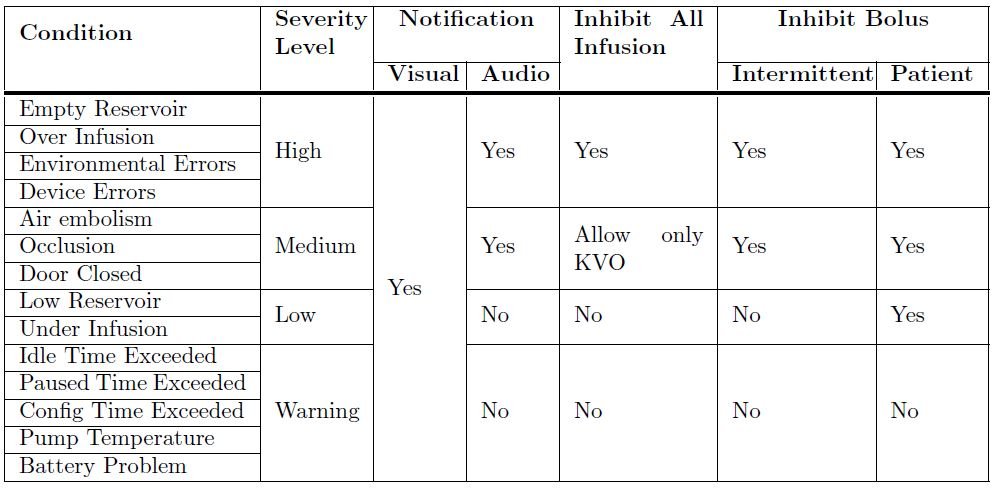
\includegraphics[width=\columnwidth]{images/alarm.jpg}
    \caption{Notification Requirements Table}
    \label{fig:gpca-alarm}
 \end{figure}


This structuring greatly helped in systematically determining the context of each requirement while formalizing it. It provided enough information about the orthogonality and exclusivity among the modes. For instance, by examining the requirements hierarchically from the top level, we were able to precisely identify and formalize the context of the patient bolus infusion requirement and the notification requirements that were discussed in Section 3.1. While such hierarchical structuring is common among modeling community, it has not been widely used to document requirements in the requirements engineering community. We believe that using such a strategy not only helps reducing the effort for formalizing requirements, but also provides the intellectual clarity to understand the system behaviours.
%%
%%such as the operating condition of the system (whether the system is ON/OFF), clinician's inputs that have influence over the entire system and the various levels of exceptional conditions documented in the alarm hierarchy requirements as shown below.
%%Infact, in some cases it helped us identify and raise the right questions to discover incomplete requirements within a hierarchical level. Overall this structuring allowed the process of formalization straightforward, that otherwise would have been an ardours trial and error approach.  %Another significant benefit of this structuring is the clarity it provides in documenting the mode transition requirements within infusion modes - descriptions about how and when transitions between those modes occur. We documented the requirements on transitions between the three modes within therapy mode, its immediate parent mode. This strategy allowed us to systematically formalize and verify the mode transition requirements -- a common source of problem in modal systems.
%%For example, the formalized requirements for patient bolus infusion was:
%\\\\
%\footnotesize{\texttt{
%SystemOn~and~not(ClinicianInhibits) and not(level2alarms and level3alams and level4alarms) and \\ \textcolor{white}{---}~and~(PatientRequest)~$\Rightarrow$ \\
%\textcolor{white}{--------}FlowRate~=~PatientFr}}
%\\\normalsize{}\\
%
%Similarly, formalizing the alarm requirements to verify them individually also became straightforward. Grouping the exceptional conditions and its associated actions in the requirements document eased the process of formalizing the requirements. We used variables (or macros) to capture the conditions that cause that alarm level and the desired actions, to avoid repetition in definitions. It then became systematic and straightforward to individually check a requirement. For example, in the GPCA there were 3 exceptional conditions that we categorized as medium level alarms, namely air in line (sensor input indicating air in infusion tube), occlusion (sensor input indicating blockage in infusion tube) and door open (sensor input indicating drug reservoir enclosure is opened). To check the door open requirement exclusively, we systematically excluded the all higher priority level alarm (HiLevelAlarm is a logical disjunction of all conditions within the highest severity level) and the other conditions in its peer level, as shown below :
%\\\\
%\footnotesize{\texttt{SystemOn and not(HiLevelAlarm) and \\
%\textcolor{white}{----}not(AirInLine) and not(Occlusion) and \\ \textcolor{white}{------}(DoorOpen)$\Rightarrow$\\
%\textcolor{white}{--------} MedLevelAlarmActions}}
%\\\normalsize{}
%


\subsection {Solution For Challenge 2: Richer Traceability}

When we identified the issue of formalizing the flow down requirements incorrectly, we started documenting a \emph{traceability argument} between requirements at adjacent levels in the hierarchy. Unlike the traditional traceability document, in which each parent level requirement is traced to its corresponding child requirement, we additionally documented an argument (a semiformal statement) explaining how the child requirement contributes to satisfying the system level requirement. This sort of assurance argument, that is inspired from Hammond's work on documenting justification for design decisions~\cite{Hammond01:WiW}, helped us understand the role of each component in satisfying the system requirement. In fact, by documenting the \emph{traceability argument} we were able to identify 8 incorrectly formalized component requirements of the GPCA. Further, this argument also helped us identify the component requirements that did not contribute to satisfying any of its parent level requirement. In sum, the traceability argument clarified the role and relevance of each requirement in satisfying its parent requirement, that in-turn helped identify the formalization errors in capturing them. To enhance the rigour of this approach, we are currently working towards building an automated traceability capability in the AGREE tool.

%
% \begin{figure}[h!]
%    \centering
%    \includegraphics[width=\columnwidth]{images/traceability.jpg}
%    \caption{Snippet from Richer Traceability Document}
%    \label{fig:gpca-alarm}
% \end{figure}


\subsection {Solution For Challenge 3: Sanity Checks and Fallibility Detection}

We believe that the root cause of the AGREE tool not identifying the consistency issues in the formalized requirements was not the tool's default setting, but the fact that it was not apparent in the results. Hence, to address the issue from the tool side we requested the tool developers to provide elaborate messages of certain key configurations when using the features, that play a key role in determining their correctness. After that change, AGREE now displays the depth of consistency check along with the results. While such a change may not be possible with every tool and feature we use, we strongly recommend the engineers to delve deep into the details and configuration of tool to precisely understand the results, especially when there is limited information provided by the tool along with the results. Additionally, this error motivated the tool developers to enhance the AGREE tool to check for \emph{vacuity}. We believe with vacuity checking we could effectively identify some of these issues. 

\subsection {Solution For Challenge 4: Automating Verifiers}

To address the transcription errors for GPCA, we first strengthened the process of verifying the translation using code inspection by a different developers. This inspection was effective in identifying errors, but was time consuming. In the long run, to maintain the synchrony between the requirements in both the tools was challenging. This challenge became the motivation for another team who are currently developing an automated translator that recaptures properties from AGREE tool notation to Embedded Matlab notation and vice-versa. While we are not actively involved in the development of the automation, we are currently verifying and validating their work using the GPCA's manual translation. While code inspections were effective, automated translators significantly reduced the overall time in the overall process. 